\section{Auswertung}
\label{sec:Auswertung}
\subsection{Wheatstonesche Brücke}
Es werden die unbekannten Widerstände mit den Werten $R_\symup{x}=\text{Wert 11}$
und $R_\symup{x}=\text{Wert 14}$ ausgemessen. Dabei treten unsystematische Fehler
bei dem Verhältnis $\frac{R_3}{R_4}$ von bis zu $\pm 0.5\%$ auf, welcher auch in
den folgenden Messungen auftritt. Da der Fehler von $R_2$ unbekannt ist, wird
dieser Widerstand dreimal variiert.
\begin{table}
  \centering
  \begin{tabular}{c c c | c c c}
  \toprule
  \multicolumn {3}{c|} {Messung für $R_{11}$} & \multicolumn {3}{c} {Messung für $R_{14}$} \\
  $R_2$ in \si{\ohm} & $R_3$ in \si{\ohm} & $R_4$ in \si{\ohm} &
  $R_2$ in \si{\ohm} & $R_3$ in \si{\ohm} & $R_4$ in \si{\ohm}\\
  \midrule
  1000 & 331 & 669  &   1000 & 475 & 525 \\
   300 & 625 & 375  &    300 & 755 & 245 \\
   644 & 427 & 573  &    644 & 577 & 423 \\
  \bottomrule
\end{tabular}
\caption{Messwerte für die Berechnung von $R_{11}$ und $R_{14}$.}
\label{tab:messwerte1}
\end{table}

Mit den bekannten Werten aus Tabelle \ref{tab:messwerte1} lassen sich mit der
Gleichung (x) die Werte der unbekannten Widerstände ausrechnen. Es ergibt sich
\begin{align*}
  R_{11} &= (491.6\pm1.4)\, \si{\ohm} \\
  R_{14} &= (902.6\pm2.6)\, \si{\ohm}.
\end{align*}


\subsection{Kapazitätsmessbrücke}
Nun werden mit einer Kapazitätsmessbrücke die unbekannten Kapazitäten
$C_\symup{x} = \text{ Wert 1}$ und $C_\symup{x} = \text{ Wert 6}$ zweier Kondensatoren,
sowie die Kapazität und der Widerstand $C_\symup{x}, R_\symup{x} = \text{ Wert 8}$
eines verlustbehafteten Kondensators bestimmt. Die Berechnung erfolgt aus den Messdaten,
die in den Tabellen \ref{tab:messwerte2} und \ref{tab:messwerte3} zu sehen sind,
und der Gleichung (x) für die Berechnung des Widerstands und der Gleichung (x)
für die Berechnung der Kapazität. Für den unbekannten Fehler von $C_2$ wird diese
Kapazität variiert.
\begin{table}
  \centering
  \begin{tabular}{c c c c | c c c c}
  \toprule
  \multicolumn {4}{c|} {Messung für $R_1$ und $C_{1}$} &
  \multicolumn {4}{c} {Messung für $R_6$ und $C_{6}$} \\
  $C_2$ in \si{\nano\farad} & $R_2$ in \si{\ohm} & $R_3$ in \si{\ohm} & $R_4$ in \si{\ohm} &
  $C_2$ in \si{\nano\farad} & $R_2$ in \si{\ohm} & $R_3$ in \si{\ohm} & $R_4$ in \si{\ohm}\\
  \midrule
  450 & 0 & 407 & 593  &  450 & 0 & 114 & 886 \\
  597 & 0 & 479 & 521  &  597 & 0 & 146 & 854 \\
  992 & 0 & 603 & 397  &  992 & 0 & 220 & 780 \\
  \bottomrule
\end{tabular}
\caption{Messwerte für die Berechnung von $R_1$, $C_{1}$ und $R_6$ und $C_{6}$.}
\label{tab:messwerte2}
\end{table}

\begin{table}
  \centering
  \begin{tabular}{c c c c}
  \toprule
  \multicolumn {4}{c} {Messung für $R_8$ und $C_8$} \\
  $C_2$ in \si{\nano\farad} & $R_2$ in \si{\ohm} & $R_3$ in \si{\ohm} & $R_4$ in \si{\ohm} \\
  \midrule
   450 & 940 & 389 & 611 \\
   597 & 910 & 391 & 609 \\
   992 & 990 & 376 & 624 \\
  \bottomrule
\end{tabular}
\caption{Messwerte für die Berechnung von $R_8$ und $C_8$.}
\label{tab:messwerte3}
\end{table}

Als Ergebnis erhält man
\begin{align*}
  R_1 &= 0 \,\si{\ohm} \\
  C_1 &= (6.53\pm0.02)\cdot10^{-7}\,\si{\farad} \\
  R_6 &= 0 \,\si{\ohm} \\
  C_6 &= (3.50\pm0.01)\cdot10^{-6}\,\si{\farad} \\
  R_8 &= (593.1\pm10.4) \,\si{\ohm} \\
  C_8 &= (1.094\pm0.003)\cdot10^{-6}\,\si{\farad}.
\end{align*}

\subsection{Induktivitätsmessbrücke}
Nachfolgend sind die Ergebnisse der Messung der Induktivität $L_\symup{x}=\text{Wert 19}$
und des Verlustwiderstands $R_\symup{x}=\text{Wert 19}$ einer unbekannten,
verlustbehafteten Spule dargestellt. Die Messwerte sind in Tabelle \ref{tab:messwerte4}
eingetragen. Mit ihnen errechnet sich $R_{19}$ nach Gleichung (x) und $L_{19}$
nach Gleichung (x).

\begin{table}
  \centering
  \begin{tabular}{c c c c}
  \toprule
  \multicolumn {4}{c} {Messung 1 für $R_{19}$ und $L_{19}$} \\
  $L_2$ in \si{\milli\henry} & $R_2$ in \si{\ohm} & $R_3$ in \si{\ohm} & $R_4$ in \si{\ohm} \\
  \midrule
   14.6 & 66 & 648 & 352 \\
   20.1 & 78 & 574 & 426 \\
  \bottomrule
\end{tabular}
\caption{Messwerte für die Berechnung von $R_{19}$ und $L_{19}$.}
\label{tab:messwerte4}
\end{table}

Somit ergeben sich bei der Messung mit der Induktivitätsmessbrücke folgende Werte:
\begin{align*}
  R_{19} &= (113.3\pm2.4)\,\si{\ohm} \\
  L_{19} &= (0.0270\pm0.0001) \,\si{\henry}
\end{align*}

\subsection{Maxwell-Brücke}
Die selbe verlustbehaftete Spule \enquote{Wert 19} wird nun ein zweites Mal mit
Hilfe einer Maxwell-Brücke ausgemessen. Die dabei gemessenen Werte sind in Tabelle
\ref{tab:messwerte5} zu sehen. Diesmal wird $R_\symup{x}=\text{Wert 19}$ mit
Gleichung (x) berechnet und $L_\symup{x}=\text{Wert 19}$ mit Gleichung (x). Da hier
wieder der Fehler von $R_2$ unbekannt ist, wird $R_2$ variiert.

\begin{table}
  \centering
  \begin{tabular}{c c c c}
  \toprule
  \multicolumn {4}{c} {Messung 2 für $R_{19}$ und $L_{19}$} \\
  $C_4$ in \si{\nano\farad} & $R_2$ in \si{\ohm} & $R_3$ in \si{\ohm} & $R_4$ in \si{\ohm} \\
  \midrule
   399 & 1000 &  69 & 640 \\
   399 &  332 & 206 & 636 \\
   399 &  664 & 104 & 639 \\
  \bottomrule
\end{tabular}
\caption{Messwerte für die Berechnung von $R_{19}$ und $L_{19}$.}
\label{tab:messwerte5}
\end{table}

Somit ergeben sich bei der Messung mit der Induktivitätsmessbrücke folgende Werte:
\begin{align*}
  R_{19} &= (107.8\pm3.2)\,\si{\ohm} \\
  L_{19} &= (0.0275\pm0.0007) \,\si{\henry}
\end{align*}
Vergleicht man dieses Ergebnis für $L_{19}$ mit dem Ergebnis, das über die
Induktivitätsmessbrücke berechnet wurde, stellt man fest, das die Werte sehr ähnlich sind.

\subsection{Wien-Robinson-Brücke}
Die Wien-Robinson-Brückenschaltung hat die Funktion eines Frequezfilters. Wertet
man die Messdaten aus Tabelle \ref{tab:messwerte6} aus, bestätigt sich die Frequenzabhänigkeit
der Brückenschaltung. Bei der Sperrfrequenz $v_0$, die sich mit
\begin{equation*}
  \omega_0 = \frac{1}{R C} = \frac{1}{1000\si{\ohm}652.7\cdot10^{-9}\si{\farad}}
  =1532.1\si{\hertz}
  \iff v_0 = \frac{\omega_0}{2\pi}=243.8 \si{\hertz}
\end{equation*}
zu $v_0 = 243.8 \si{\hertz}$ ergibt, sollte die Ausgangsspannung verschwinden.

\begin{table}
  \centering
  \begin{tabular}{r r r}
  \toprule
  v in \si{\hertz} & $U_{Br}$ in \si{\volt} & $U_S$ in Volt \\
  \midrule
  20    &  2.38  &  7.44\\
  40    &  2.22  &      \\
  60    &  1.94  &      \\
  80    &  1.62  &      \\
  100   &  1.3   &      \\
  150   &  0.7   &      \\
  180   &  0.44  &      \\
  200   &  0.3   &      \\
  210   &  0.2   &      \\
  220   &  0.14  &      \\
  230   &  0.08  &      \\
  240   &  0.02  &  7.12\\
  250   &  0.08  &      \\
  260   &  0.15  &      \\
  270   &  0.16  &      \\
  300   &  0.36  &      \\
  350   &  0.58  &      \\
  400   &  0.8   &      \\
  500   &  1.11  &      \\
  1000  &  1.92  &      \\
  2000  &  2.16  &  6.8 \\
  5000  &  2.24  &      \\
  10000 &  2.16  &      \\
  15000 &  2.16  &      \\
  20000 &  2.16  &      \\
  30000 &  2.08  &  6.4 \\
\end{tabular}
\caption{Messwerte der Wien-Robinson-Brücke.}
\label{tab:messwerte6}
\end{table}
Der experimentell bestimmte Wert für die Sperrfrequenz beträgt $v_0 = 240 \si{\hertz}$.
Der Wert hat eine relative Abweichung von $\Delta v_{0,rel} = 1.23 \%$ zum
Theoriewert und ist damit gut bestimmt.
\begin{figure}
  \centering
  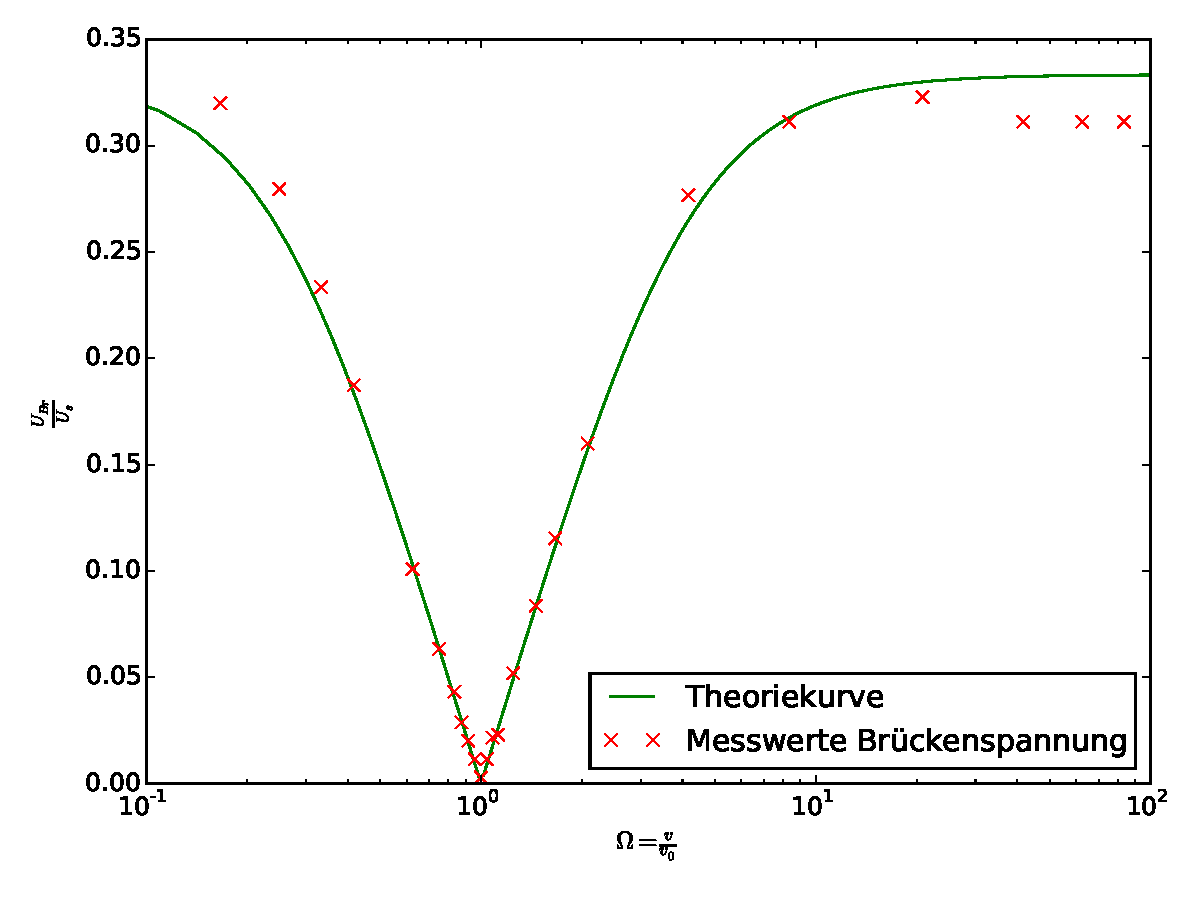
\includegraphics[width=0.9\textwidth]{wien-robinson.pdf}
  \caption{Messwerte und Theoriekurve der Wien-Robinson-Brücke.}
  \label{fig:wien-robinson}
\end{figure}
In Grafik \ref{fig:wien-robinson} zeigt sich, dass insbesondere in der näheren
Umgebung um $v_0$, die Messwerte sehr gut mit der Theoriekurve (x) übereinstimmen.
Frequenzen mit $v \leq 40 \si{\hertz}$ oder $v \geq 15000 \si{\hertz}$ weichen
jedoch deutlich von der Theoriekurve ab.

\subsection{Klirrfaktor-Messung}
Zur Bestimmung des Klirrfaktor des verwendeten Generators wird die vereinfachende
Annahme getroffen, dass die Brückenspannung, die bei der Sperrfrequenz
$v_0=243.8 \si{\hertz}$ noch gemessen werden kann - also die Summe der Amplituden
der  Oberwellen - nur aus denen zweiten Oberwellen besteht.
Mit Gleichung (x) wird zunächst die Spannung $U_2$ berechnet:
\begin{equation*}
  \frac{U_{Br}(v_0)}{f(2)} = \frac{0.02\si{\volt}}{\sqrt{\frac{1}{45}}} = 0.134 \si{\volt}.
  \label{eqn:U2}
\end{equation*}
Für den Klirrfaktor ergibt sich damit nach Gleichung (x):
\begin{equation*}
  k = \frac{U_2}{U_1} = \frac{0.134 \si{\volt}}{7.12\si{\volt}} = 0.0188 \si{\volt}
  \label{eqn:klirrfaktor_berechnung}
\end{equation*}
